\hyphenation{ra-dia-tion}
\hyphenation{re-gu-la-ri-ty}
\hyphenation{thres-hold}
\hyphenation{ge-ne-ra-li-za-tion}
\chapter{Event generation, simulation and reconstruction}\label{ch:gensimreco}

\section{Introduction}

The process of analyzing data recorded by the CMS experiment involves several stages where the data are processed in order to interpret the information provided by all the detection systems; in those stages, the particles produced after the \pp collision are identified by reconstructing their trajectories and measuring their features. In addition, the SM provides a set of predictions that have to be compared with the experimental results; however, in most of the cases, theoretical predictions are not directly comparable to experimental results due to the diverse source of uncertainties introduced by the experimental setup and theoretical approximations, among others.

The strategy to face these conditions consists in using statistical methods implemented in computational algorithms to produce numerical results that can be contrasted with the experimental results. These computational algorithms are commonly known as Monte Carlo (MC) methods and, in the case of particle physics, they are designed to apply the SM rules and produce predictions about the physical observables measured in the experiments. Since particle physics is governed by quantum mechanics principles, predictions are not allowed from single events; therefore, a high number of events are \ti{generated} and predictions are produced in the form of statistical distributions for the observables. Effects of the detector presence are included in the predictions by introducing simulations of the detector itself.     

This chapter presents a description of the event generation strategy and the tools used to perform the detector simulation and physics objects reconstruction. A comprehensive review of event generators for LHC physics can be found in Reference \cite{gen} on which this chapter is based.  

\section{Event generation}\label{sec:event_generation}

\begin{figure}[!h]
  \centering
  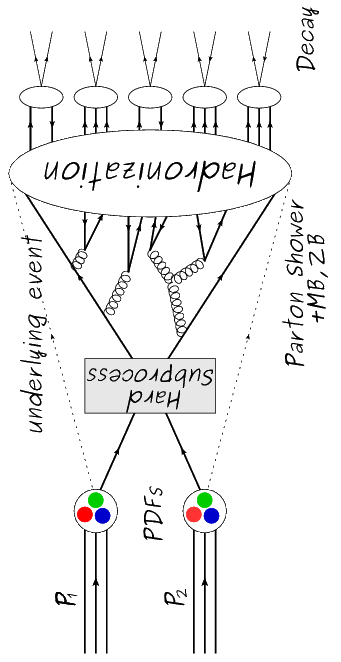
\includegraphics[scale=0.6,angle=-90]{gen}
  \caption[Event generation process.]{Event generation process. %In the first step, the PDF of the colliding particles is considered so the specific interaction is described.
    The actual interaction is generated in the hard subprocess%; the cross-section of the process is calculated from the matrix element connecting the initial and final states
    . The parton shower describes the evolution of the partons from the hard subprocess.% according to the DGLAP equations. At this step, the underlying event and PU effects are included in the generation. The resulting partons from the parton shower are recombined to form hadrons in the hadronization step; most of them are unstable, therefore, their decays are also generated in agreement to the known branching ratios.
     Modified from Reference \cite{gen_scheme}.}\label{fig:gen}
\end{figure}

The event generation is intended to create events that mimic the behavior of actual events produced in collisions; they obey a sequence of steps from the particles collision hard process to the decay process into the final state. Figure \ref{fig:gen} shows a schematic view of the event generation process; the fact that the full process can be treated as several independent steps is motivated by the QCD factorization theorem.     

Generation starts by taking into account the PDFs of the incoming particles. Event generators offer the option to chose from several PDF sets depending on the particular process under simulation\footnote{Tool in Reference \cite{pdfplot} allows to plot different PDF sets under customizable conditions.}; in the following, \pp collisions will be considered. The \textit{hard subprocess} describes the actual interaction between partons from the incoming protons; it is represented by the matrix element connecting the initial and final states of the interaction. Normally, the matrix element can be written as a sum over Feynman diagrams and consider interferences between terms in the summation. During the generation of the hard subprocess, the production cross section is calculated. 

The order to which the cross section is calculated depends on the order of the Feynman diagrams involved in the calculation; therefore, radiative corrections are included by considering a higher order Feynman diagrams where QCD radiation dominates. Currently, cross sections calculated to LO do not offer a satisfactory description of the processes, \ie, the results are only reliable for the shape of distributions; therefore, NLO calculations have to be performed with the implication that the computing time needed is highly increased.       

The final parton content of the hard subprocess is subjected to the \textit{parton shower} which generates the gluon radiation. Parton shower evolves the partons, \ie, glouns split into quark-antiquark pairs and quarks with enough energy radiate gluons giving rise to further parton multiplication, following the DGLAP (Dokshitzer-Gribov-Lipatov-Altarelli-Parisi) equations \cite{dglap1,dglap2,dglap3}. Showering continues until the energy scale is low enough to reach the non-perturbative limit.   

In the simulation of LHC processes that involve $b$ quarks, like the single top quark or Higgs associated production, it is needed to consider that the $b$ quark is heavier than the proton; hence, the QCD interaction description is made in two different schemes \cite{schemes}

\begin{itemize}

\item four-flavor (4F) scheme. $b$ quarks appear only in the final state because they are heavier than the proton and therefore they can be produced only from the splitting of a gluon into pairs or singly in association with a $t$ quark in high energy-scale interactions; furthermore, during the simulation, the $b$-PDFs are set to zero. Calculations in this scheme are more complicated due to the presence of the second $b$ quark but the full kinematics is considered already at LO and therefore the accuracy of the description is better.   

\item five-flavor (5F) scheme. $b$ quarks are considered massless, therefore they can appear in both initial and final states since they can now be part of the proton; thus, during the simulation $b$-PDFs are not set to zero. In this scheme, calculations are simpler than in the 4F scheme and possible logarithmic divergences are absorbed by the PDFs through the DGLAP evolution.   
\end{itemize}

In this thesis, the \tHq events are generated using the 4F scheme in order to reduce uncertainties, while the \tHW events are generated using the 5F scheme to eliminate LO interference with \ttH process\cite{demartin}.    

Partons involved in the \pp collision are the focus of the simulation, however, the rest of the partons inside the incoming protons are also affected because the remnants are colored objects; also, multiple parton interactions can occur. The hadronization of the remnants and multiple parton interactions are known as \ti{underlying event} and it has to be included in the simulation. In addition, multiple \pp collisions in the same bunch crossing (pile-up mentioned in \ref{sec:lhc}) occurs, actually in two forms

\begin{itemize}
\item \textit{in-time PU} which refers to multiple \pp collision in the bunch crossing but that are not considered as primary vertices. 
\item \textit{Out-of-time PU} which refers to overlapping \pp collisions from consecutive bunch crossings; this can occur due to the time-delays in the detection systems where information from one bunch crossing is assigned to the next or previous one. 
\end{itemize}

While the underlying event effects are included in generation using generator-specific tools, PU effects are added to the generation by overlying Minimum-bias (MB) and Zero-bias (ZB) events to the generated events. MB events are inelastic events selected by using a loose trigger with as little bias as possible, therefore accepting a large fraction of the overall inelastic event; ZB events correspond to random events recorded by the detector when collisions are likely. MB models in-time PU and ZB models out-of-time PU. 

The next step in the generation process is called \ti{hadronization}. Since particles with a net color charge are not allowed to exits isolated, they have to recombine to form bound states. This is precisely the process by which the partons resulting from the parton shower arrange themselves as color singlets to form hadrons. At this step, the energy-scale is low and the strong coupling constant is large, therefore hadronization process is non-perturbative and the evolution of the partons is described using phenomenological models. Most of the baryons and mesons produced in the hadronization are unstable and hence they will decay in the detector.

The last step in the generation process corresponds to the decay of the unstable particles generated during hadronization; it is also simulated in the hadronization step, based on the known branching ratios. 

\section{Monte Carlo Event Generators.}

The event generation described in the previous section has been implemented in several software packages for which a brief description is given.     

\begin{itemize}

\item \textbf{PYTHIA 8}. It is a program designed to perform the generation of high energy physics events which describes the collisions between particles such as electrons and protons. Several theories and models are implemented in it, in order to describe physical aspects like hard and soft interaction, parton distributions, initial and final-state parton showers, multiple parton interactions, beam remnants, hadronization\footnote{based in the Lund string model \cite{lund}} and particle decay. Thanks to extensive testing, several optimized parametrizations, known as \ti{tunings}, have been defined in order to improve the description of actual collisions to a high degree of precision; for analysis at $\sqrt{s}=13$ TeV, the underline event CUETP8M1 tune is employed \cite{tune}.  The calculation of the matrix element is performed at LO which is not enough for the current required level of precision; therefore, pythia is often used for parton shower, hadronization and decays, while other event generators are used to generate the matrix element at NLO.
\item \textbf{MadGraph5\_aMC@NLO}. MadGraph is a matrix element generator which calculates the amplitudes for all contributing Feynman diagrams of a given process but does not provide a parton shower while MC@NLO incorporates NLO QCD matrix elements consistently into a parton shower framework; thus, MadGraph5\_aMC@NLO, as a merger of the two event generators MadGraph5 and aMC@NLO, is an event generator capable to calculate tree-level and NLO cross sections and perform the matching of those with the parton shower. It is one of the most frequently used matrix element generators; however, it has the particular feature of the presence of negative event weights which reduce the number of events used to reproduce the properties of the objects generated \cite{madgraph}.
\item \textbf{POWHEG}. It is an NLO matrix element generator where the hardest emission of color charged particles is generated in such a way that the negative event weights issue of MadGraph5\_aMC@NLO is overcome; however, the method requires an interface with  $p_T$-ordered parton shower or a parton shower generator where this highest emission can be vetoed in order to avoid double counting of this highest-energetic emission. PYTHIA is a commonly matched to POWHEG event generator \cite{powheg}.
\end{itemize}

Events resulting from the whole generation process are known as MC events. 

\section{CMS detector simulation.}

After generation, MC events contain the physics of the collisions but they are not ready to be compared to the events recorded by the experiment since these recorded events correspond to the response of the detection systems to the interaction with the particles traversing them. The simulation of the CMS detector has to be applied on top of the event generation; it is simulated with a MC toolkit for the simulation of particles passing through matter called Geant4 which is also able to simulate the electronic signals that would be measured by all detectors inside CMS.   

The simulation takes the generated particles contained in the MC events as input, makes them pass through the simulated geometry, and models physics processes that particles experience during their passage through matter. The full set of results from particle-matter interactions corresponds to the simulated hit which contains information about the energy loss, momentum and position. Particles of the input event are called \ti{primary}, while the particles originating from GEANT4-modeled interactions of a primary particle with matter are called a \ti{secondary}.  Simulated hits are the input of subsequent modules that emulate the response of the detector readout system and triggers. The output from the emulated detection systems and triggers is known as digitization \cite{geant,geant2}.

The modeling of the CMS detector corresponds to the accurate modeling of the interaction among particles, the detector material, and the magnetic field. This simulation procedure includes the following standard steps
\begin{itemize}
\item Modeling of the Interaction Region.
\item Modeling of the particle passage through the hierarchy of volumes that compose CMS detector and of the accompanying physics processes.
\item Modeling of the effect of multiple interactions per beam crossing and/or the effect of events overlay ( Pile-Up simulation).
\item Modeling of the detector's electronics response, signal shape, noise, calibration constants (digitization). 
\end{itemize}

In addition to the full simulation, \ie, a detailed detector simulation, a faster simulation (FastSim) have been developed, that may be used where much larger statistics are required. In FastSim, detector material effects are parametrized and included in the hits; those hits are used as input of the same higher-level algorithms\footnote{track fitting, calorimeter clustering, b tagging, electron identification, jet reconstruction and calibration, trigger algorithms which will be considered in the next sections} used to analyze the recorded events. In this way, comparisons between fast and full simulations can be performed \cite{fastsim}.

After the full detector simulation, the output events can be directly compared to events actually recorded in the CMS detector. The collection of MC events that reproduces the expected physics for a given process isknown as MC sample.

\section{Event reconstruction.}

%In contrast to MC samples for which all the particles' information is available from its identity to its mass and energy, recorded events contain the electronic signals, provided by the CMS detection systems, encoding the interaction of physical particles with the detector matter; these electronic signals have to be combined in order to identify these particles and measure their features, \ie, particles have to be \ti{reconstructed} using the signals provided by the detection systems.
The CMS experiment use the \ti{particle-flow event reconstruction algorithm (PF)} to do the reconstruction of particles produced in \pp collisions. Next sections will present a basic description of the \textit{Elements} used by PF (tracker tracks, energy clusters, and muon tracks), based in the References \cite{particle_flow, particle_flow2} where more detailed descriptions can be found.  

\subsection{Particle-Flow Algorithm.}\label{subsec:particle_flow}

Each of the several sub detection systems of the CMS detector is dedicated to identify an specific type of particles, \ie, photons and electrons are absorbed by the ECAL and their reconstruction is based on ECAL information; hadrons are reconstructed from clusters in the HCAL while muons are reconstructed from hits in the muon chambers. PF is designed to correlate signals from all the detector layers (tracks and energy clusters) in order to reconstruct and identify each final state particle and its properties as sketched in Figure \ref{fig:pf}.

\begin{figure}[!h]
  \centering
  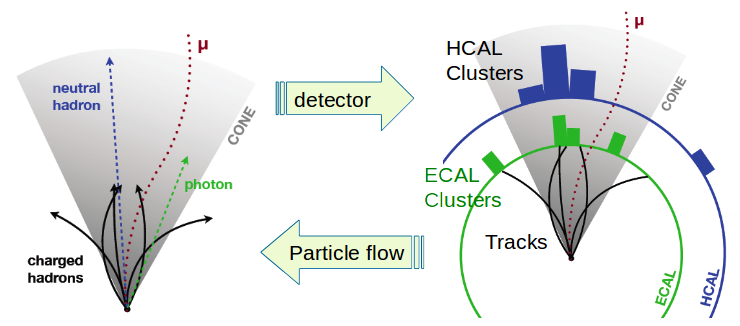
\includegraphics[width=\textwidth]{pf}
  \caption[Particle flow algorithm.]{Particle flow algorithm. Information from the several CMS detection systems if provided as input to the algorithm which then combine it to identify and reconstruct all the particles in the final state and their properties. Reconstruction of simulated events is also performed by providing information from MC samples, detector and trigger simulation \cite{pfdiag}.}\label{fig:pf}
\end{figure}

For instance, a charged hadron is identified by a geometrical connection, known as \textit{link}, between one or more calorimeter clusters and a track in the tracker, provided there are no hits in the muon system; combining several measurements allows a better determination of the energy and charge sign of the charged hadron.   


\subsubsection*{Charged-particle track reconstruction.}

The strategy used by PF in order to reconstruct tracks is called \ti{Iterative Tracking} which occurs in four steps

\begin{itemize}
\item Seed generation where initial track candidates are found by looking for a combination of hits in the pixel detector, strip tracker, and muon chambers. In total ten iterations are performed, each one with a different seeding requirement. Seeds are used to estimate the trajectory parameters and uncertainties at the time of the full track reconstruction. Seeds are also considered track candidates.    
\item Track finding using a tracking software known as Combinatorial Track Finder (CTF) \cite{ctf}. The seed trajectories are extrapolated along the expected flight path of a charged particle, in agreement to the trajectory parameters obtained in the first step, in an attempt to find additional hits that can be assigned to the track candidates. 
\item Track-fitting where the found tracks are passed as input to a module which provides the best estimate of the parameters of each trajectory.
\item Track selection where track candidates are submitted to a selection which discards those that fail a set of defined quality criteria.
\end{itemize}

Iterations differ in the seeding configuration and the final track selection as elaborated in References \cite{particle_flow, particle_flow2}. In the first iteration, high \pt tracks and tracks produced near to the interaction region are identified and those hits are masked thereby reducing the combinatorial complexity. Next, iterations search for more complicated tracks, like low \pt tracks and tracks from b hadron decays, which tend to be displaced from the interaction region.

\subsubsection*{Vertex reconstruction.}

During the track reconstruction, an extrapolation toward to the calorimeters is performed in order to match energy deposits; that extrapolation is performed also toward the beamline in order to find the origin of the track known as \textit{vertex}. The vertex reconstruction is performed by selecting from the available reconstructed tracks, those that are consistent with being originated in the interaction region where \pp collisions are produced. The selection involves a requirement on the number of tracker (pixel and strip) hits and the goodness of the track fit.

Selected tracks are clustered using a \ti{deterministic annealing algorithm (DA)}\footnote{DA algorithm and AVF are described in detail in References \cite{da, avf}}. A set of candidate vertices and their associated tracks, resulting from the DA, are then fitted with an \ti{adaptive vertex fitter (AVF)} to produce the best estimate of the vertices locations.

The \pt of the tracks associated to a reconstructed vertex is added, squared and used to organize the vertices; the vertex with the highest squared sum is designated as the \textit{primary vertex (PV)} while the rest are designated as PU vertices. 

\subsubsection*{Calorimeter clustering.}

After traversing the CMS tracker system, electrons, photons and hadrons deposit their energy in the ECAL and HCAL cells. The PF clustering algorithm aims to provide a high detection efficiency even for low-energy particles and an efficient distinction between close energy deposits. The clustering runs independently in the ECAL barrel and endcaps, HCAL barrel and endcaps, and the two preshower layers, following two steps
\begin{itemize}
\item cells with an energy larger than a given seed threshold and larger than the energy of the neighboring cells are identified as cluster seeds. The neighbor cells are those that either share a side with the cluster seed candidate, or the eight closest cells including cells that only share a corner with the seed candidate.
\item cells with at least a corner in common with a cell already in the cluster seed and with an energy above a cell threshold are grouped into topological clusters.
\end{itemize}

Clusters formed in this way are known as \textit{particle-flow clusters}. With this clustering strategy, it is possible to detect and measure the energy and direction of photons and neutral hadrons as well as differentiate these neutral particles from the charged hadron energy deposits. In cases involving charged hadrons for which the track parameters are not determined accurately, for instance, low-quality and high-\pt tracks, clustering helps in the energy measurements. 

\subsubsection*{Electron track reconstruction.}

Although the charged-particle track reconstruction described above works for electrons, they lose a significant fraction of their energy via bremsstrahlung photon radiation before reaching the ECAL; thus, the reconstruction performance depends on the ability to measure also the radiated energy. The reconstruction strategy, in this case, requires information from the tracking system and from the ECAL. Bremsstrahlung photons are emitted at similar \etac values to that of the electron but at different values of \phic; therefore, the radiated energy can be recovered by grouping ECAL clusters in a \etac window over a range of \phic around the electron direction. The group is called ECAL supercluster (SC) .

Electron candidates from the track-seeding and ECAL super clustering are merged into a single collection which is submitted to a full electron tracking fit with a Gaussian-sum filter (GSF) \cite{gsf}. The electron track and its associated ECAL supercluster form a \textit{particle-flow electron}.

\subsubsection*{Muon track reconstruction.}

Given that the CMS detector is equipped with a muon spectrometer capable to identify and measure the momentum of the muons traversing it, the muon reconstruction is not specific to PF; therefore, three different muon types are defined

\begin{itemize}
\item \textit{Standalone muon}. A clustering on the DTs or CSCs hits is performed to form track segments; those segments are used as seeds for the reconstruction in the muon spectrometer. All DTs, CSCs, and RPCs hits along the muon trajectory are combined and fitted to form the full track. The fitting output is called a \textit{standalone-muon track}.
\item \textit{Tracker muon}. Each track in the inner tracker with \pt larger than 0.5 GeV and a total momentum $p$ larger than 2.5 GeV is extrapolated to the muon system. A \textit{tracker muon track} corresponds to a extrapolated track that matches at least one muon segment.
\item \textit{Global muon}. When tracks in the inner tracker (inner tracks) and ${\textrm{standalone-muon}}$ tracks are matched and turn out being compatibles, their hits are combined and fitted to form a \textit{global-muon track}. 
\end{itemize}

Global muons sharing the same inner track with tracker muons are merged into a single candidate. PF muon identification uses the muon energy deposits in ECAL, HCAL, and HO associated with the muon track to improve the muon identification.

\subsubsection*{Particle identification and reconstruction.} \label{subsubsec:part_id_reco}

PF elements are connected by a linker algorithm that tests the connection between any pair of elements; if they are found to be linked, a geometrical distance that quantifies the quality of the link is assigned. Two elements may be linked indirectly through common elements. Linked elements form \textit{PF blocks} and each PF block may contain elements originating in one or more particles. Links can be established between tracks, between calorimeter clusters, and between tracks and calorimeter clusters. The identification and reconstruction start with a PF block and proceed as follows     

\begin{itemize}

\item Muons. An \ti{isolated global muon} is identified by evaluating the presence of inner track and energy deposits close to the global muon track in the (\etac,\phic) plane, \ie, in a particular point of the global muon track, inner tracks and energy deposits are sought within a radius of $\Delta R=0.3$ (see eqn. \ref{delta_r}) from the muon track; if they exit and the \pt of the found track added to the \Et of the found energy deposit does not exceed 10\% of the muon \pt then the global muon is an isolated global muon. This isolation condition is stringent enough to reject hadrons misidentified as muons.

  \ti{Non-isolated global muons} are identified using additional selection requirements on the number of track segments in the muon system and energy deposits along the muon track. Muons inside jets are identified with more stringent criteria in isolation and momentum as described in Reference \cite{muon_req}. The PF elements associated with an identified muon are masked from the PF block.  

\item Electrons are identified and reconstructed as described above plus some additional requirements on fourteen variables like the amount of energy radiated, the distance between the extrapolated track position at the ECAL and the position of the associated ECAL supercluster, among others, which are combined in an specialized multivariate analysis strategy that improves the electron identification.

There are three methods for charge estimation; one is the sign of the curvature of the GSF track; a second method is based on matching a CTF track to a GSF track when at least one hit is shared in the innermost region. In the third method, the vector joining the beam spot and the SC position and the vector joining the beam spot and the first hit of the electron GSF track, are compared; the charge is estimated from the sign of the difference in \phic between these two vector. The electron charge is defined by the sign shared by at least two of the three estimates \cite{mva_eid1}.
  
Tracks and clusters used to identify and reconstruct electrons are masked in the PF block.  
  
\item Isolated photons are identified from ECAL superclusters with \Et larger than 10 GeV, for which the energy deposited at a distance of 0.15, from the supercluster position on the (\etac,\phic) plane, does not exceed 10\% of the supercluster energy; note that this is an isolation requirement. In addition, there must not be links to tracks. Clusters involved in the identification and reconstruction are masked in the PF block.

\item Bremsstrahlung photons and prompt photons tend to convert to electron-positron pairs inside the tracker, therefore, a dedicated finder algorithm is used to link tracks that seem to originate from a photon conversion; in case those two tracks are compatible with the direction of a bremsstrahlung photon, they are also linked to the original electron track. Photon conversion tracks are also masked in the PF block.

\item The remaining elements in the PF block are used to identify hadrons. In the region $|\eta| \leq 2.5$, neutral hadrons are identified with HCAL clusters not linked to any track while photons from neutral pion decays are identified with ECAL clusters without links to tracks. In the region $|\eta| >2.5$ ECAL clusters linked to HCAL clusters are identified with a charged or neutral hadron shower; ECAL clusters with no links are identified with photons.
  HCAL clusters not used yet, are linked to one or more unlinked tracks and to an unlinked ECAL in order to reconstruct charged-hadrons or a combination of photons and neutral hadrons according to certain conditions on the calibrated calorimetric energy.         

\item Charged-particle tracks may be liked together when they converge to a \ti{secondary vertex (SV) } displaced from the IP where the PV and PU vertices are reconstructed; at least three tracks are needed in that case, of which at most one has to be an incoming track with hits in tracker region between a PV and the SV.
\end{itemize}

The linker algorithm, as well as the whole PF algorithm, has been validated and commissioned; results from that validation are presented in the Reference \cite{particle_flow}.

\subsubsection*{Jet reconstruction.}

Quarks and gluons may be produced in the \pp collisions, therefore, their hadronization will be seen in the detector as a shower of hadrons and their decay products in the form of a \ti{jet}. Two classes of clustering algorithms have been developped based in their jet definition \cite{coco}:  

\bit
\item Iterative cone algorithms (IC). Jets are defined in terms of circles of fixed radius $R$ in the \etac-\phic plane, known as \ti{stable cones}, for which the sum of the momenta of all the particles within the cone points in the same direction as the center of the circle. The seed of the iteration is the hardest non-isolated particle in the event, then, the resulting momentum direction is assigned as the new cone direction and a new iteration starts; iteration process stops when the cone if found to be stable. 
\item Sequential recombination algorithms. The distance between non-isolated particles is calculated; if that distance is below a threshold, these particles are recombined into a new object. The sequence is repeated until the separation between the recombined object and any other particle is above certain threshold; the recombined object is called a jet and the algorithm starts again with the remaining particles.      
\eit

\begin{figure}[!h]
  \centering
  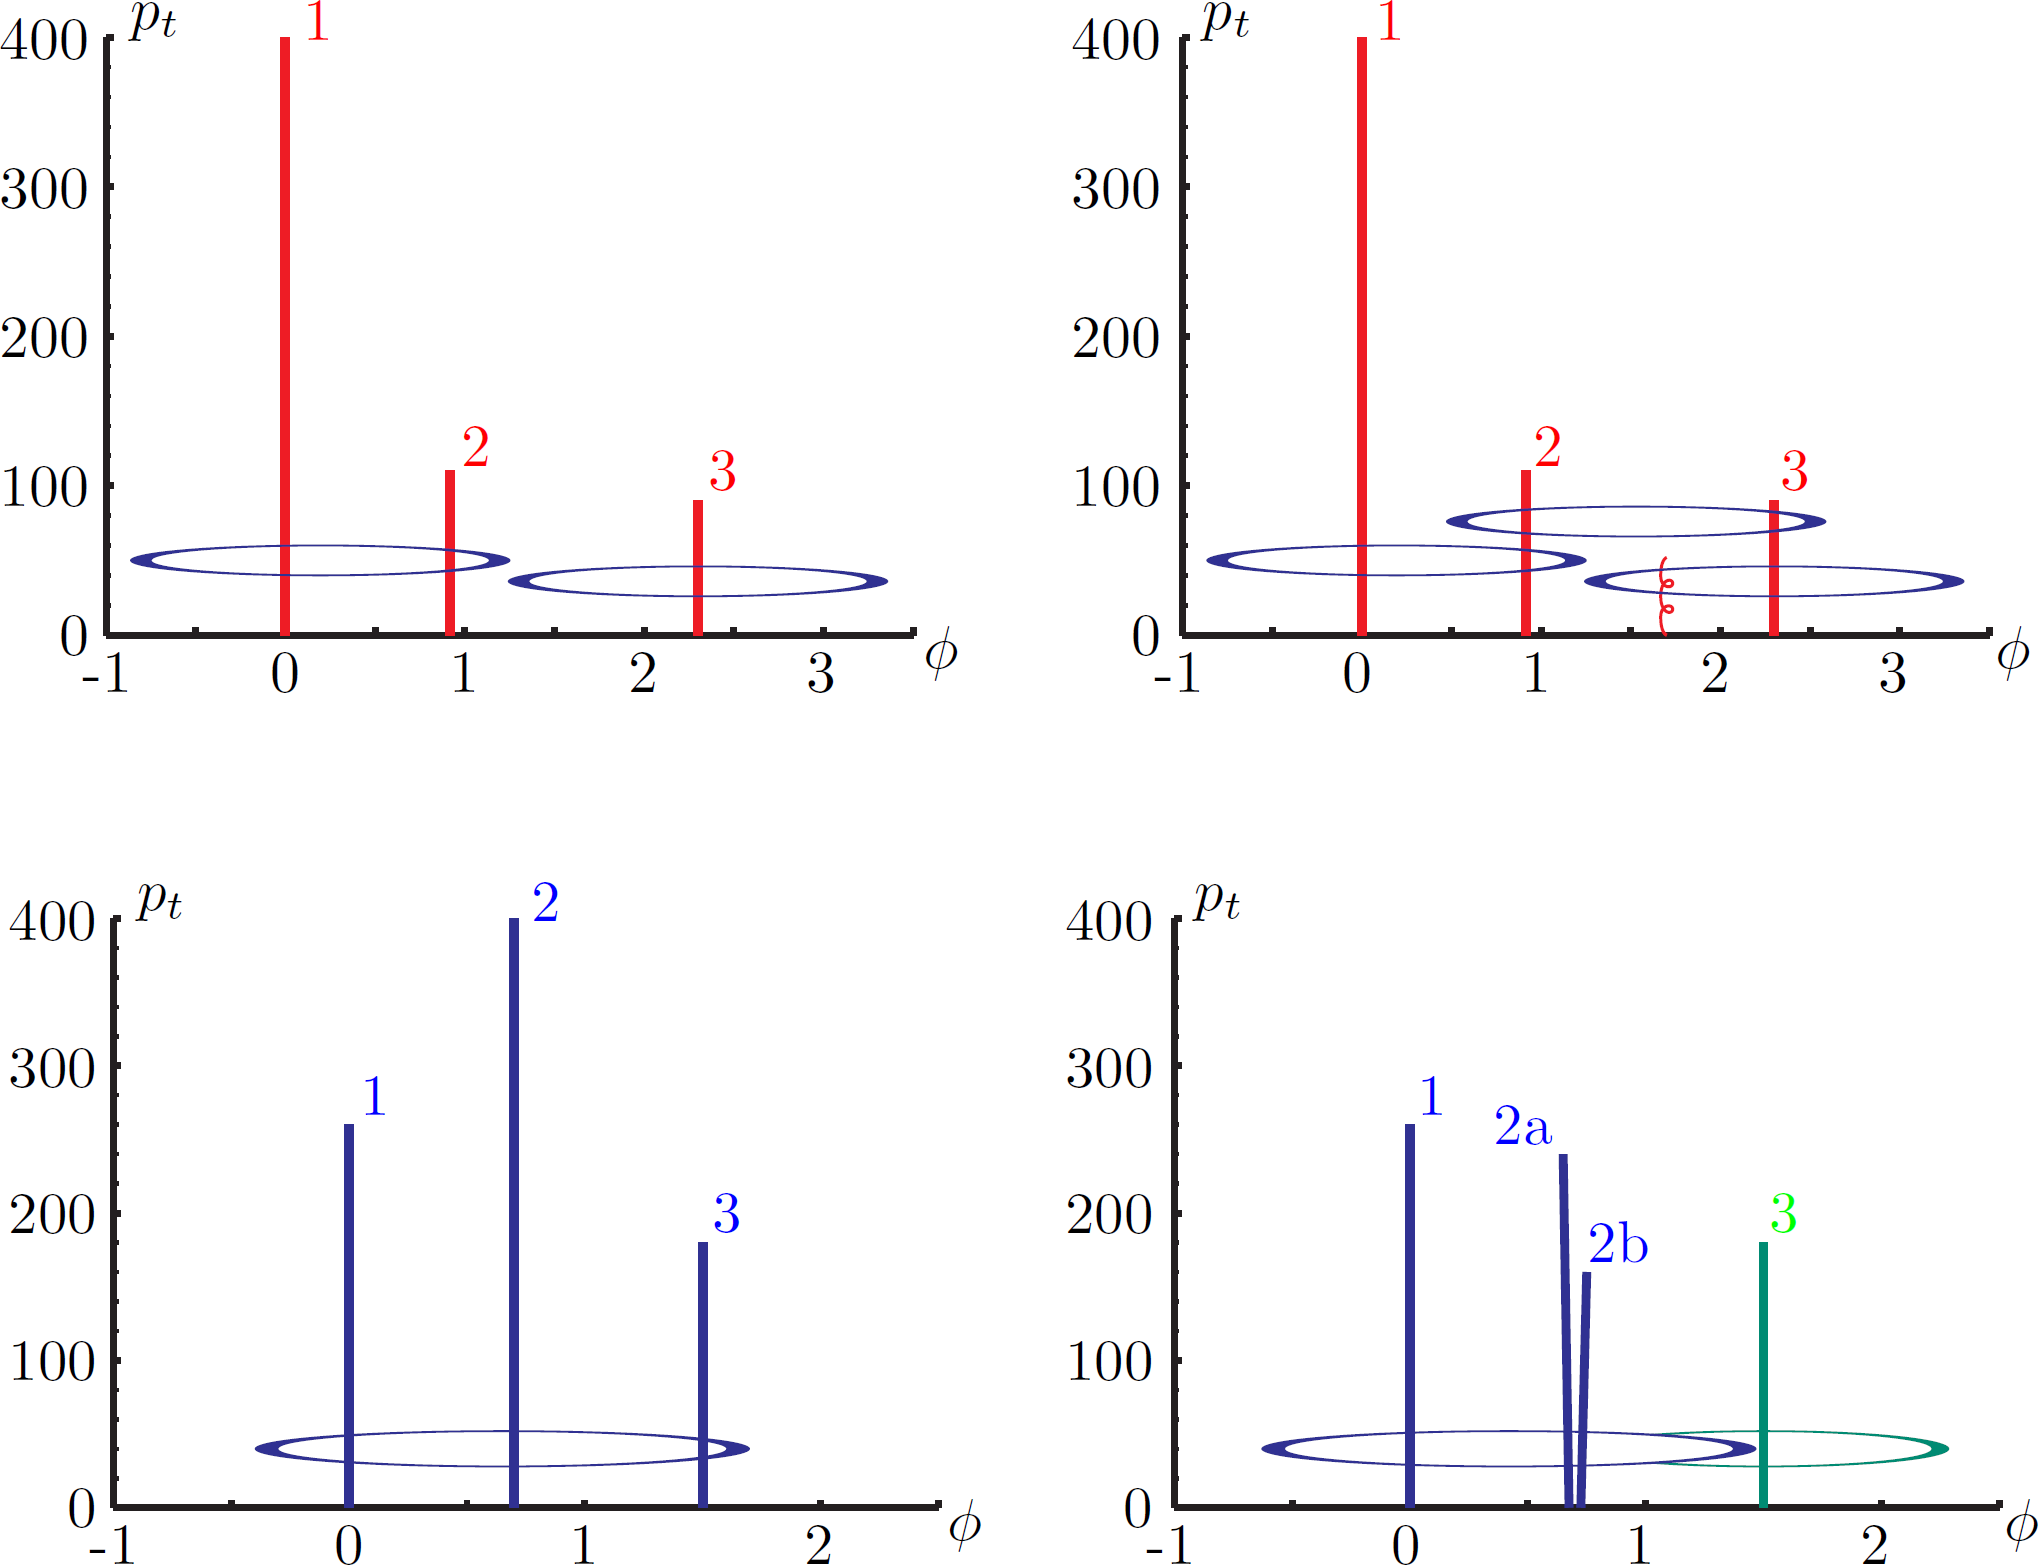
\includegraphics[scale=0.25]{ircs}
  \caption[Stable cones identification]{Stable cones identification using IC algorithms \cite{coco}.}\label{fig:irc}
\end{figure}

Two conditions are of particular importance for the clustering algorithms, \ti{infrared and collinear (IRC) safety}. In order to explain the concept of infrared (IR) safety, consider an event with three hard particles as shown in the top left side of Figure \ref{fig:irc}, two stable cones are found and then two jets are identified; if a soft gluon is added, as shown in the top right side of Figure \ref{fig:irc}, three stable cones are found and the three hard particles are now clustered into a single jet. If the addition of soft particles change the outcome of the clustering, then it is said that the algorithm is IR unsafe. Soft radiation is highly likely in perturbative QCD, which dominates the physics of the jets, and then IR unsafe effect leads to divergences \cite{coco}.

The concept of collinear safety can also be explained considering a three hard particles event, as shown in the bottom left side of Figure \ref{fig:irc}, where one stable cone containing all three particles is found and one jet is identified; if the hardest particle is split into two collinear particles (2a and 2b) in the bottom right side of Figure \ref{fig:irc}, then the clustering results in a different jet identification and the algorithm is said to be collinear unsafe. The collinear unsafe effect leads to divergences in jet cross section calculations \cite{antikt}.       

It has been determined that IC algorithms are IRC unsafe, and therefore, they have to be replaced by algorithms that not only provide the finite perturbative results from theoretical computations, but also that are not highly dependent on underlying event and pileup effects which leads to significant corrections\cite{coco}.

The sequential recombination algorithms arise as the IRC safe alternative used by the CMS experiment; in particular the anti-$k_t$ algorithm\cite{antikt} which is a generalization of the previously existing $k_t$ \cite{kt} and Cambridge/Aachen \cite{ac} jet clustering algorithms.

The anti-$k_t$ algorithm is used to perform the jet reconstruction by clustering those PF particles within a cone (see Figure \ref{fig:jetcone}); previously, isolated electrons, isolated muons, and charged particles associated with other interaction vertices are excluded from the clustering.  

\begin{figure}[!h]
  \centering
  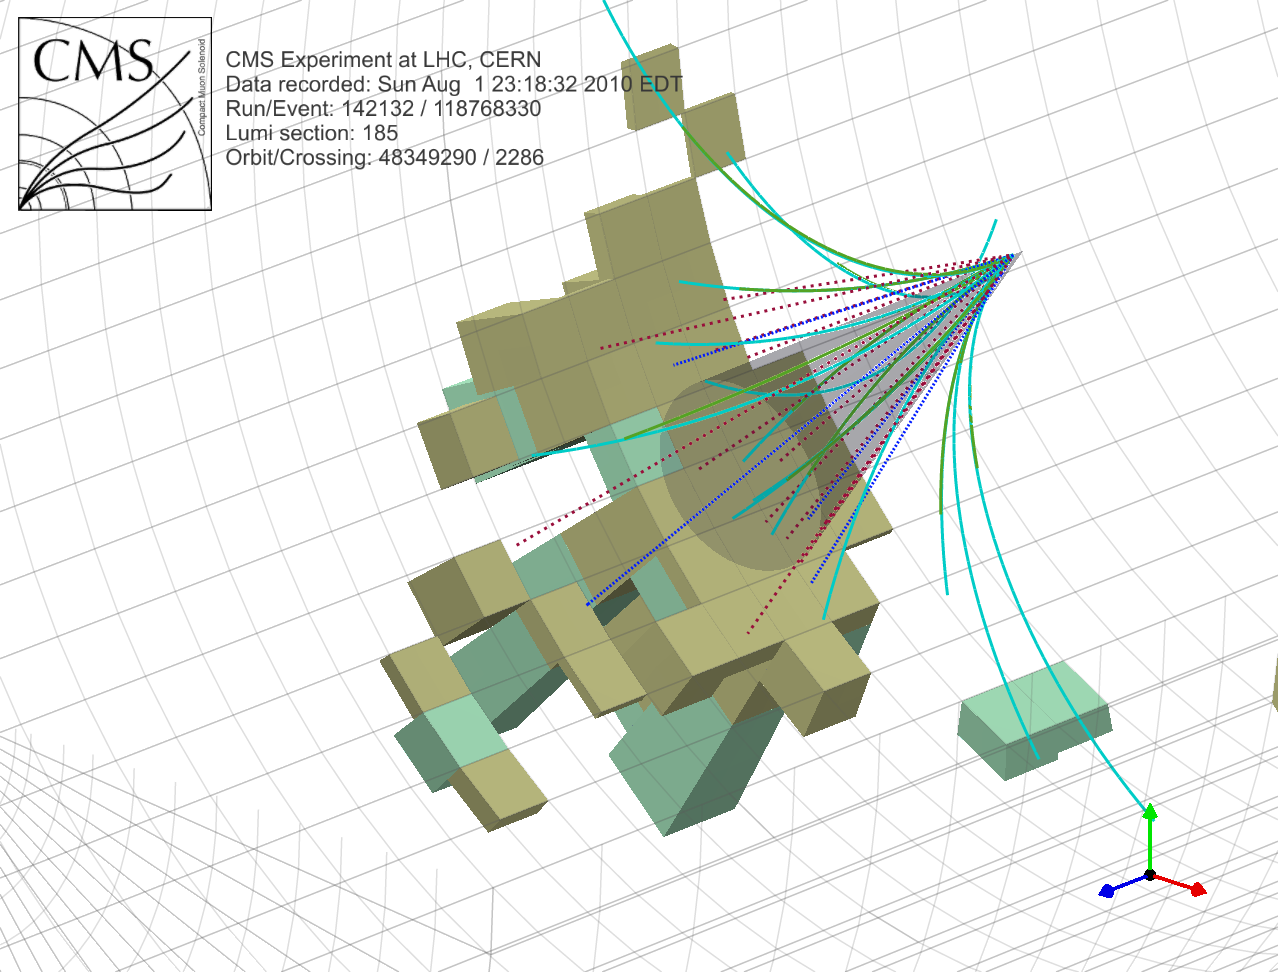
\includegraphics[width=7.5cm, height=5cm]{JetConeAll}
  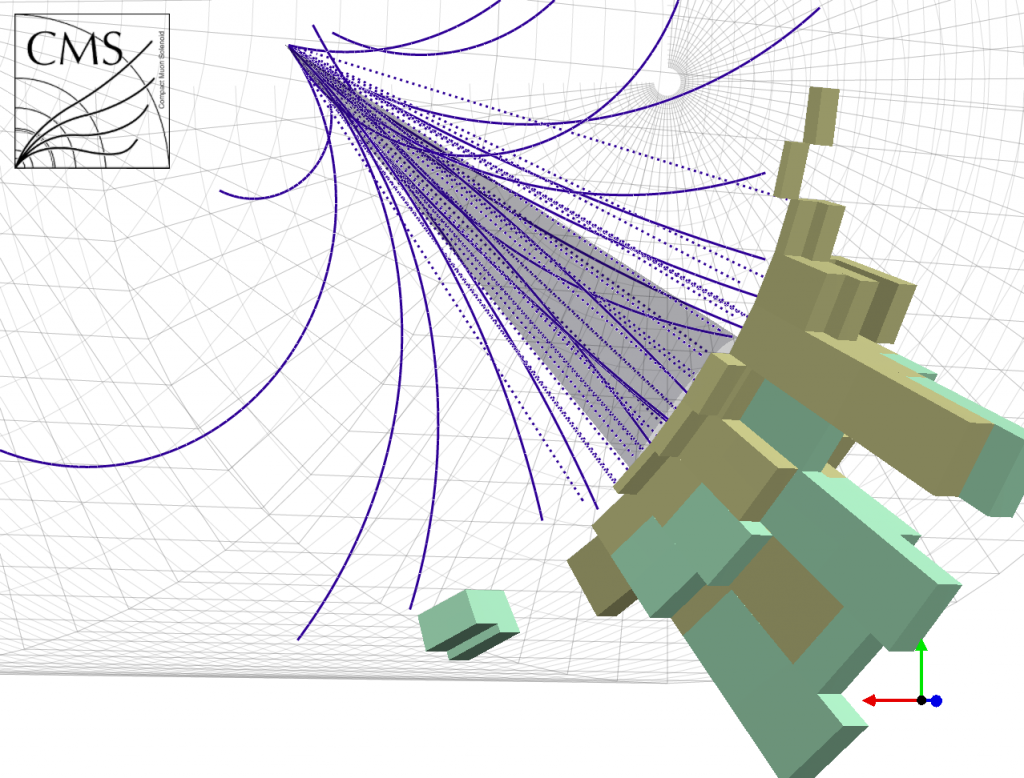
\includegraphics[width=7.5cm, height=5cm]{JetConeAll2}
    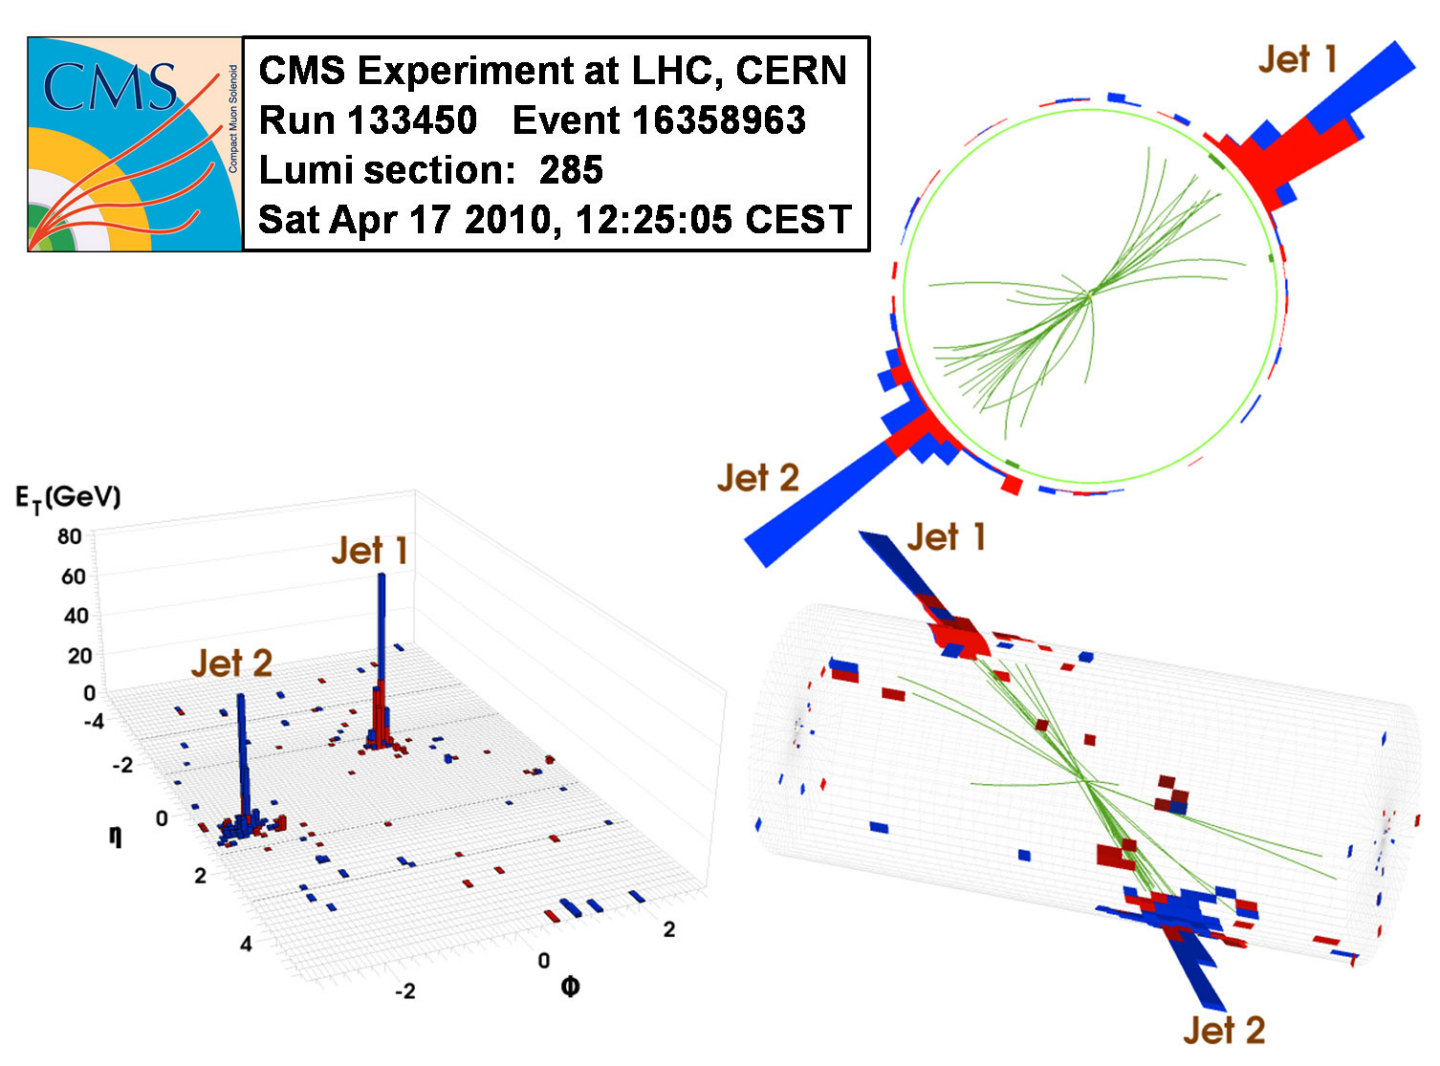
\includegraphics[width=7.5cm, height=5cm]{jetreco}
  \caption[Jet reconstruction.]{Jet reconstruction performed by the anti-$k_t$ algorithm. Top: Two different views of a CMS recorded event are presented. Continuous lines correspond to tracks left by charged particles in the tracker while dotted lines are the imaginary paths followed by neutral particles. The green cubes represent the ECAL cells while the blue ones represent the HCAL cells; in both cases, the height of the cube represent the amount of energy deposited in the cells \cite{jetconeview}. Bottom: Reconstruction of a recorded event with two jets \cite{jetreco}.}\label{fig:jetcone}
\end{figure}

The anti-$k_t$ algorithm proceeds in a sequential recombination of PF particles; the distance between particles $i$ and $j$ ($d_{ij}$)  and the distance between particles and the beam are defined as

\begin{align}\label{cov_der}
  d_{ij} = & \textrm{min}\left(\frac{1}{k_{ti}^2},\frac{1}{k_{tj}^2}\right)\frac{\Delta_{ij}^2}{R^2} \nonumber\\
  d_{iB} = & \frac{1}{k_{ti}^2}
\end{align}

\noindent where $\Delta_{ij}^2=(y_i-y_j)^2 + (\phi_i-\phi_j)^2$, $k_{ti}, y_i$ and $\phi_i$ are the transverse momentum, rapidity and azimuth of particle $i$ respectively and R is the called jet radius. For all the remaining PF particles, after removing the isolated ones, $d_{ij}$ and $d_{iB}$ are calculated\footnote{Notice that this is a combinatorial calculation.} and the smallest is identified; if it is a $d_{ij}$, particles $i$ and $j$ are replaced with a new object whose momentum is the vectorial sum of the combined particles. If the smallest distance is a $d_{iB}$ the clustering process ends, the object $i$ (which at this stage should be a combination of several PF particles) is declared as a \textit{Particle-flow-jet} (PF jet) and all the associated PF particles are removed from the detector. The clustering process is repeated until no PF particles remain. R is a free parameter that can be adjusted according to the specific analysis conditions; usually, two values are used, R=0.4 and R=0.5, giving the name to the so-called AK4-jet and AK5-jet respectively.     

An advantage of the anti-$k_t$ algorithm over other clustering algorithms is the regularity of the boundaries of the resulting jets. For all known IRC safe algorithms, soft radiation can introduce irregularities in the boundaries of the final jets; however, anti-$k_t$ algorithm is soft-resilient, meaning that jets shape is not affected by soft radiation, which is a valuable property considering that knowing the typical shape of jets makes experimental calibration of jets more simple. In addition, that soft-resilience is expected to simplify certain theoretical calculations and reduce the momentum-resolution loss caused by underlying-event (UE) and pileup contamination \cite{antikt}.  

The effect of the UE and pileup contamination over a jet identification, can be seen as if soft events are added to the jet; for instance, if a soft event representing UE or pileup is added to an event for which a set of jets J have been identified, and the clustering is rerun on that new extended event, the outcome will be different in two aspects: jets will contain some additional soft energy and the distribution of particles in jets may have change; that effect is called \ti{back-reaction}. The back-reaction effect in the anti-$k_t$ algorithm is suppressed not by the amount of momentum added to the jet but by the jet transverse momentum $p_{T,J}$, which means that this strong suppression leads to a smaller correction due to EU and pileup effect\cite{antikt}.               


\subsubsection*{Jet energy Corrections}

\begin{figure}[!h]
  \centering
  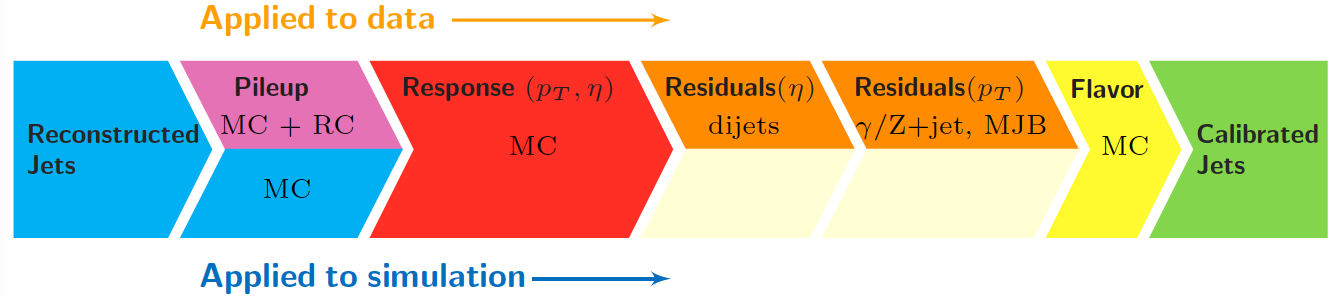
\includegraphics[width=\textwidth]{jec}
  \caption[Jet energy corrections.]{Jet energy correction diagram. Correction levels are applied sequentially in the indicated fixed order \cite{jec2}.}\label{fig:jec}
\end{figure}

Even though jets can be reconstructed efficiently, there are some effects that are not included in the reconstruction and that lead to discrepancies between the reconstructed results and the predicted results; in order to overcome these discrepancies, a factorized model has been designed in the form of jet energy corrections (JEC) \cite{jec,jec2} applied  sequentially as shown in the diagram of Figure \ref{fig:jec}.

At each level, the jet four-momentum is multiplied by a scaling factor based on jet properties, \ie, \etac, flavor, etc.

\begin{itemize}
\item Level 1 correction removes the energy coming from pile-up. The scale factor is determined using a MC sample of QCD dijet (2 jets) events with and without pileup overlay; it is parametrized in terms of the offset energy density $\rho$, jet area A, jet \etac and jet \pt. Different corrections are applied to data and MC due to the detector simulation.
\item MC-truth correction accounts for differences between the reconstructed jet energy and the MC particle-level energy. The correction is determined on a QCD dijet MC sample and is parametrized in terms of the jet \pt and \etac.
\item Residuals correct remaining small differences within jet response in data and MC. The Residuals \etac-dependent correction compares jets of similar \pt in the barrel reference region. The Residuals \pt-dependent correct the jet absolute scale (JES vs \pt).
\item Jet-flavor corrections are derived in the same way as MC-truth corrections but using QCD pure flavor samples. 
\end{itemize}  

\subsubsection*{$b$-tagging of jets.}

A particular feature of the hadrons containing bottom quarks (b-hadrons) is that their lifetime is long enough to travel some distance before decaying, but it is not as long as those of light quark hadrons; therefore, when looking at the hadrons produced in \pp collisions, b-hadrons decay typically inside the tracker rather than reaching the calorimeters as some light-hadrons do. As a result, a b-hadron decay gives rise to a displaced vertex (secondary vertex) with respect to the primary vertex as shown in Figure \ref{fig:sv}; the SV displacement is in the order of a few millimeters. A jet resulting from the decay of a b-hadron is called $b$ jet; other jets are called light jets. 

\begin{figure}[!h]
  \centering
  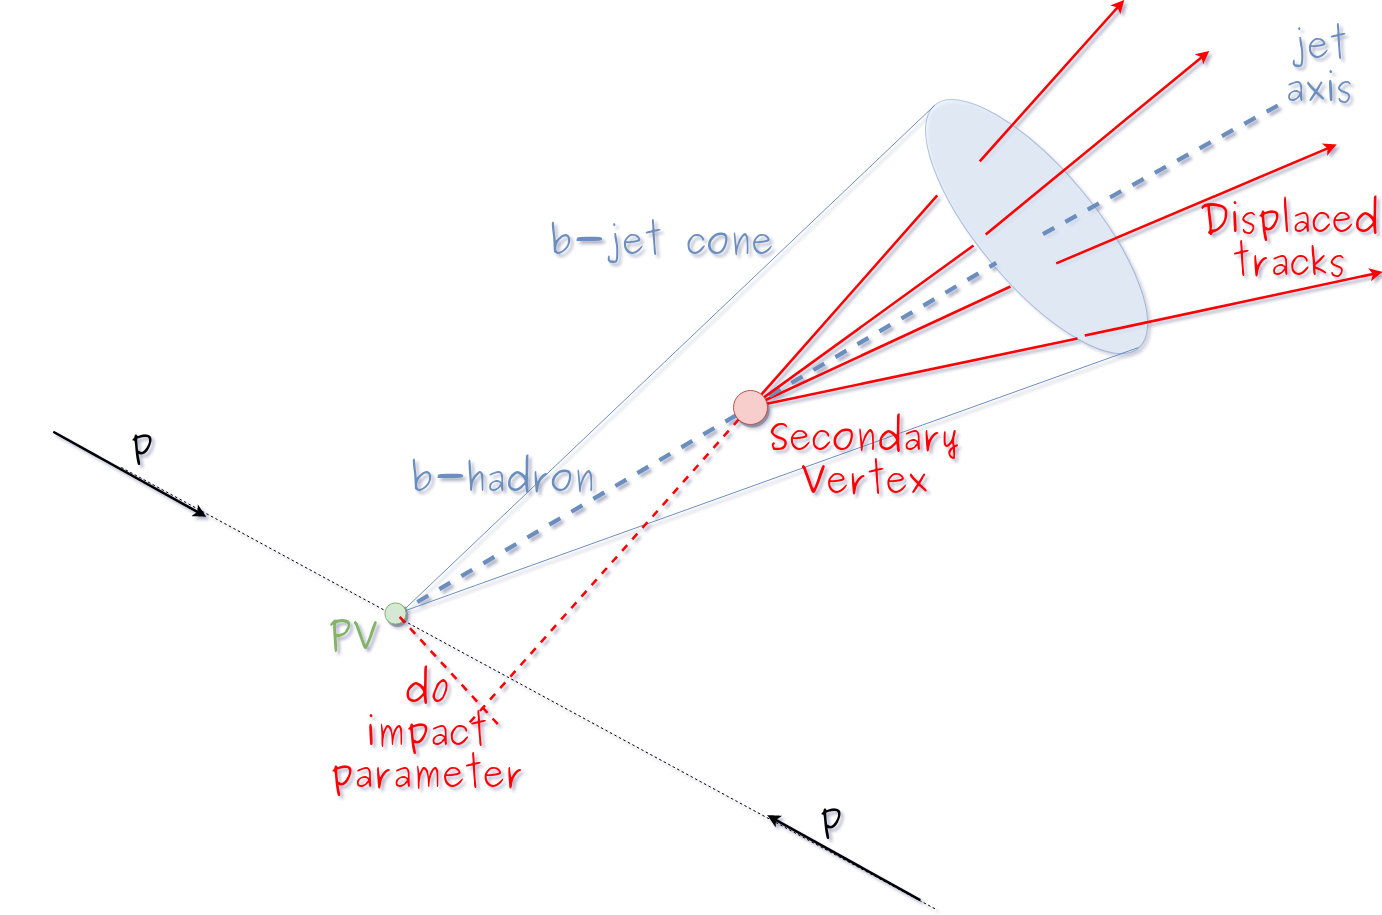
\includegraphics[scale = 0.3]{sv}
  \caption[Secondary vertex in a b-hadron decay.]{Secondary vertex in a b-hadron decay.}\label{fig:sv}
\end{figure}

Several methods to identify $b$-jets ($b$-tagging) have been developed; the method used in this thesis is known as \ti{Combined Secondary Vertex} algorithm in its second version (CSVv2) \cite{btag}. By using information of the impact parameter, the reconstructed secondary vertices, and the jet kinematics as input in a multivariate analysis that combines the discrimination power of each variable in one global discriminator variable, three working points (references): loose, medium and tight, are defined which quantify the probabilities of mistag jets from light quarks as jets from $b$ quarks; 10, 1 and 0.1 \% respectively. Although the mistagging probability decreases with the working point strength, the efficiency to correctly tag $b$-jets also decreases as 83, 69 and 49 \% for the respective working point; therefore, a balance needs to be achieved according to the specific requirements of the analysis.

\subsubsection*{Missing transverse energy.}\label{sssec:met}

The fact that proton bunches carry momentum along the $z-$axis implies that for each event it is expected that the momentum in the transverse plane is balanced. Imbalances are quantified by the missing transverse energy (MET) and are attributed to several sources including particles escaping undetected through the beam pipe, neutrinos produced in weak interactions processes which do not interact with the detector and thus escaping without leaving a sign, or even undiscovered particles predicted by models beyond the SM.

The PF algorithm assigns the negative sum of the momenta of all reconstructed PF particles to the \textit{particle-flow MET} according to
\beqn
\vec{\slashed{E}}_T=-\sum_{i}\vec{p}_{T,i}
\eeqn
JEC are propagated to the calculation of the $\vec{\slashed{E}}_T$ as described in the Reference \cite{metcorr}.

\subsection{Event reconstruction examples}

Figure \ref{fig:reco1} shows the results of the reconstruction performed on a recorded event. The cmsShow-10.0 tool \cite{cmsshow} have been used to produce these images.  The event recorded was with the CMS detector in 2016 at a proton-proton center-of-mass energy of 13 TeV; it shows the characteristics expected from the decay of the SM Higgs boson to a pair of $W$ bosons with the subsequent production of two muons. A third lepton is observed in the central region of the detector and identified as the decay product of a third W boson. The expected forward jet and \bjet are also clearly visible, while the violet arrow represent the presence of MET.

Figure \ref{fig:reco3} shows the $\rho$-z projection of the event in Figure \ref{fig:reco1}; The displaced reconstructed vertex (the secondary vertex) where the $b$ quark is produced is marked by a black dot; it iis tagged by CSVv2T algorithm. The number of reconstructed primary vertices is 13 (shown in orange color dots). Beam spot position correction is applied.

\begin{figure}[!h]
\vspace{-1cm}
  \centering
  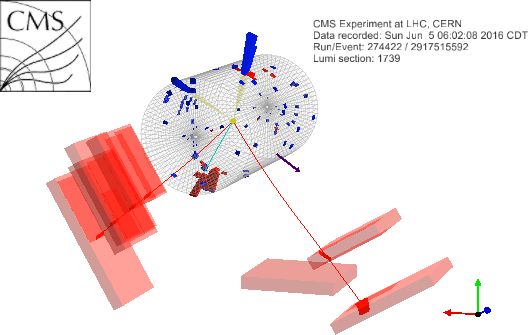
\includegraphics[width=0.8\textwidth]{3d_thq_event1.png}
  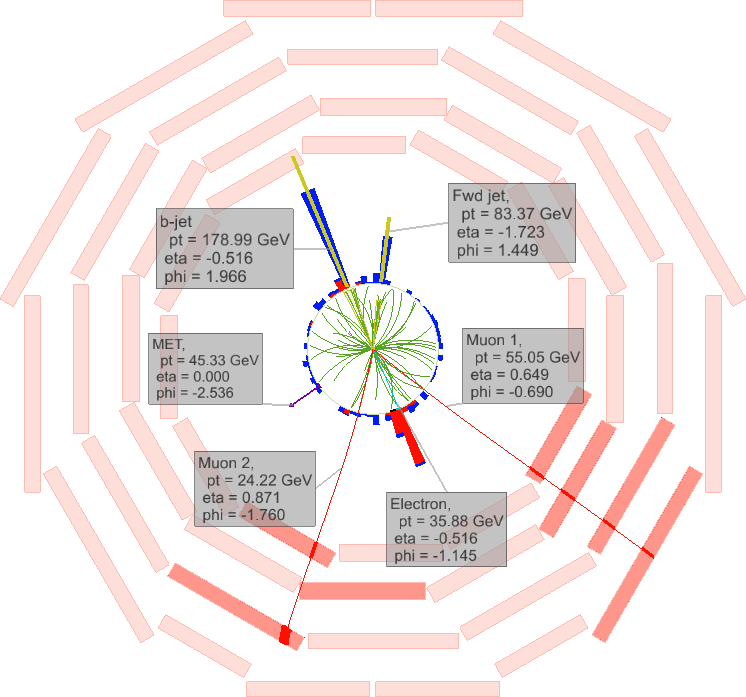
\includegraphics[width=0.9\textwidth]{rho_phi_thq_event1.png}        
  \caption[\tHq Event reconstruction.]{\tHq Event reconstruction results}\label{fig:reco1}
\end{figure}

\begin{landscape}
\begin{figure}[h]
  \centering
  \vspace{-2cm}
  \hspace{-1cm}
  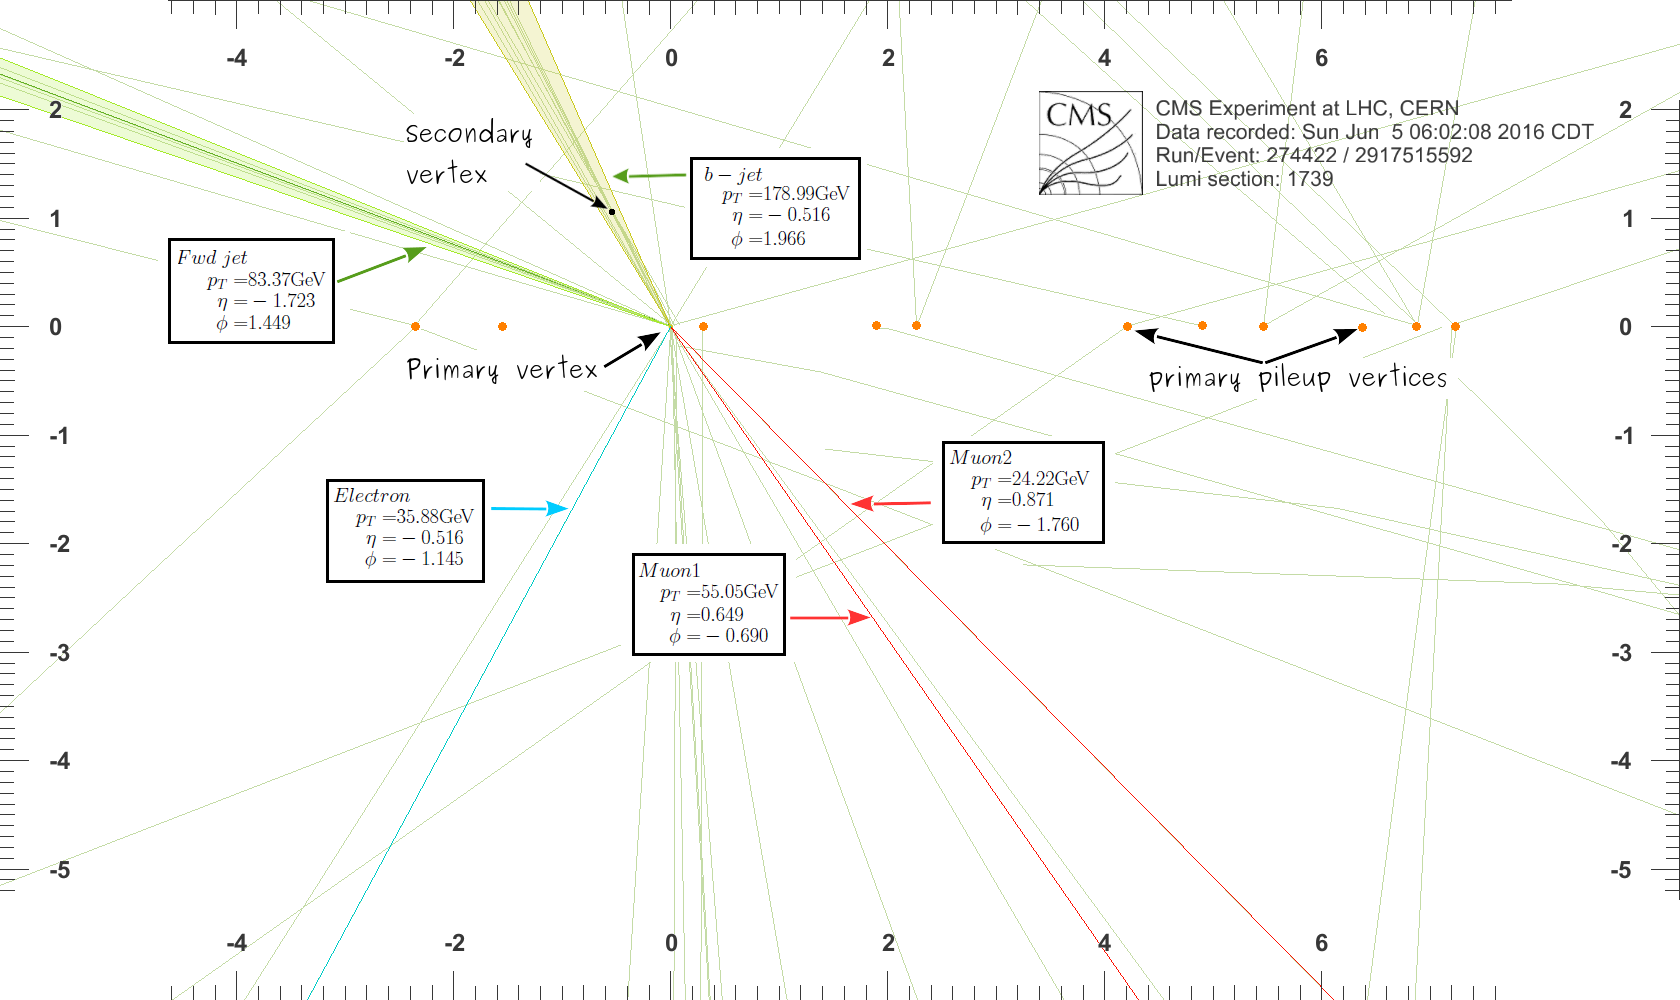
\includegraphics[width=23cm,height=15.2cm]{rho_z_thq_event1.png}
  \caption[Event close-up view with the multiple interactions.]{Event close-up view with the multiple interactions. }\label{fig:reco3}  
  \vspace{-1cm}
  \hspace{-2cm}
  \end{figure}
\end{landscape}
